\documentclass[a4paper,10pt]{article}

\usepackage{tikz}
\usepackage{xltxtra}
\usepackage{dirtree}
\usepackage{graphicx}
\usepackage{hyperref}
\usepackage{csquotes}\usepackage{listings}
\usepackage{pgfplots}
\usepackage[
backend=biber,
style=alphabetic,
sorting=ynt
]{biblatex}
\pgfplotsset{compat=1.17}
\addbibresource{bib.bib}
\hypersetup{
    colorlinks=true,
    linkcolor=blue,
    filecolor=magenta,
    urlcolor=cyan,
}
\lstset{
    frame=single,
    captionpos=b,
}

\setsansfont[Mapping=tex-text]{Source Sans 3}
\setromanfont[Mapping=tex-text]{Source Serif 4}
\setmonofont[Mapping=tex-text]{Source Code Pro}

\title{OpenBSD: Segurança Inovadora em SOs}
\author{Pedro Igor Martins dos Reis}
\date{\today}

\begin{document}
\begin{titlepage}
    \centering
    {\Huge\bfseries OpenBSD: Segurança e Inovação em Sistemas Operacionais\par}
    \vspace{2cm}
    {\Large Gustavo Valadares Castro\par}
    {\Large Hernane Velozo Rosa\par}
    {\Large João Martins Medeiros\par}
    {\Large Pedro Igor Martins dos Reis\par}
    \vspace{2cm}
    {\large \today\par}
    \vfill
    
\includegraphics[width=0.3\textwidth]{imagens/logo_pucminas.png}\par\vspace{1cm}
    {\large Pontifícia Universidade Católica de Minas Gerais\par}
    {\large Instituto de Ciências Exatas e Informática\par}
\end{titlepage}
\section{Introdução}
OpenBSD é um sistema operacional de código aberto derivado do Berkeley Software Distribution (BSD), uma versão do sistema operacional UNIX.
O projeto OpenBSD foi iniciado em 1995 por Theo de Raadt, um programador do Canadá que também foi um dos fundadores do projeto NetBSD. O OpenBSD é conhecido e respeitado por seu foco em aspectos como proatividade, correção de código e segurança.
\begin{figure}[!ht]
    \centering
    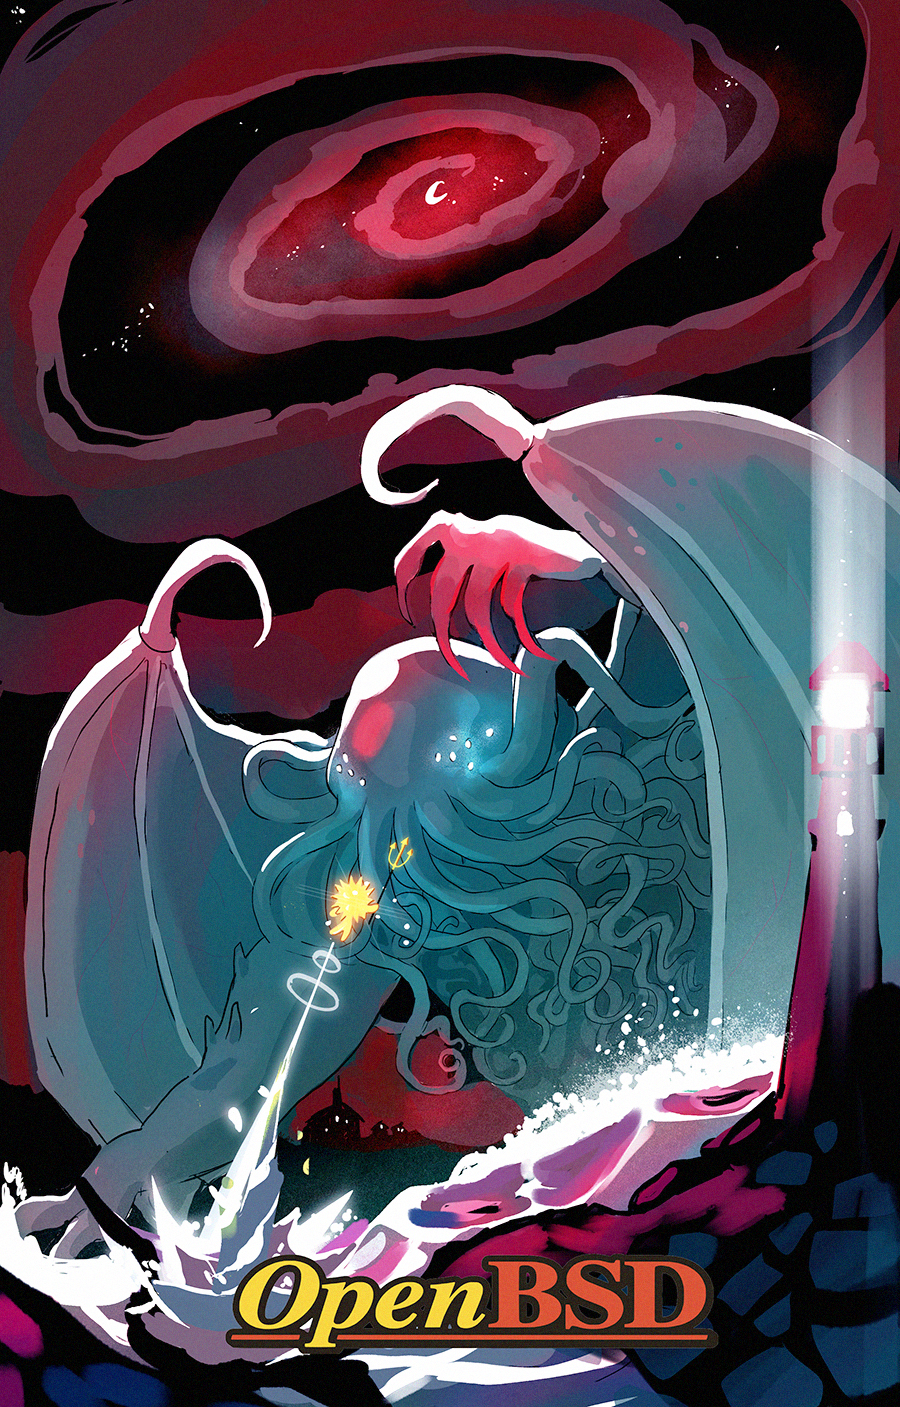
\includegraphics[width=0.5\textwidth]{imagens/puffy_vs_cthulhu.jpg}
    \caption{Arte de fãs para o OpenBSD}
\end{figure}

\subsection{Filosofia do projeto}
A filosofia do OpenBSD é fornecer um sistema operacional simples, completo, seguro e de alta qualidade. O sistema se destaca pela quantidade significativa de código que seus desenvolvedores criam, bem como pela meticulosa atenção aos detalhes e à segurança durante o desenvolvimento. O OpenBSD inclui uma série de recursos de segurança ausentes ou opcionais em outros sistemas operacionais, tornando-o uma escolha popular para situações que exigem alta segurança, como firewalls, sistemas de prevenção de intrusões e servidores.

O OpenBSD também é conhecido por sua documentação de alta qualidade. Cada programa no sistema vem com um manual que descreve em detalhes suas funcionalidades, opções e instruções de uso. Isso torna o OpenBSD um excelente ambiente de aprendizado para pessoas interessadas em sistemas operacionais UNIX e BSD.

Além disso, o projeto OpenBSD produziu vários componentes de software de alta qualidade que foram adotados por outros sistemas operacionais. O mais notável deles é o OpenSSH, o pacote de software de rede criptografado mais amplamente utilizado em todo o mundo.

\subsection{Breve história do OpenBSD}

Em relação à história do OpenBSD, a primeira versão foi lançada em outubro de 1995 por Theo de Raadt como um fork da versão 1.0 do \href{https://www.netbsd.org/}{NetBSD}. Theo de Raadt é não apenas o fundador e líder do projeto, mas também foi responsável pelo desenvolvimento do OpenSSH. A principal motivação por trás do projeto foi devido a divergências de Theo com a equipe do NetBSD, da qual ele fazia parte.

\begin{figure}[!ht]
    \centering
    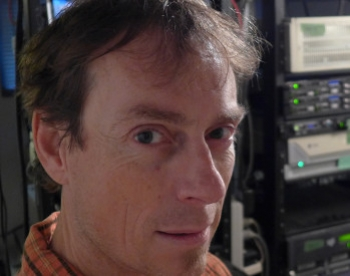
\includegraphics[width=0.5\textwidth]{imagens/thao-de-raadt.jpg}
    \caption{Theo de Raadt}
\end{figure}

Desde 1995, o OpenBSD tem lançado regularmente várias versões do sistema operacional a cada 6 meses. Essa estabilidade torna o OpenBSD ideal e amplamente utilizado em servidores que lidam com sistemas críticos, como e-mail, FTP, DNS e muitos outros. O projeto tem mantido um progresso consistente em direção aos seus objetivos, que serão explorados com mais detalhes ao longo deste texto.

Em 2007, Bob Beck, um dos membros do projeto OpenBSD, anunciou
a formação da OpenBSD Foundation. Essa fundação foi estabelecida com o fim de representar, quando necessário, não apenas o projeto OpenBSD principal, mas também outros projetos relacionados, como OpenSSH, OpenBGPD, OpenNTPD, OpenCVS, LibreSSL etc.A OpenBSD Foundation foi criada para facilitar e coordenar contribuições e patrocínios destinados a essas iniciativas, proporcionando um controle mais organizado e eficiente.

\subsection{Propósito e objetivos}
\begin{displayquote}
    \begin{center}
        \textit{Try to be the \#1 most secure operating system.}
    \end{center}
\end{displayquote}
De forma bastante didática e simples, é explicado os 10 principais objetivos do projetos, em suma, focam nos princípios da liberdade, correção do código, proatividade e principalmente segurança. Para manter-se previsível, foi estabelecido o padrão de lançamento semestral, além disto, é importante que seja mantido para o máximo de arquiteturas disponíveis:
\begin{itemize}
    \item Digital Alpha (alpha)
    \item AMD64 (amd64)
    \item 64-bit ARM (arm64)
    \item ARM v7 (armv7)
    \item HP Precision Architecture (hppa)
    \item Intel i386 (i386)
    \item IO-DATA Landisk (landisk)
    \item Loongson 2E/2F (loongson)
    \item Omron LUNA88K(2) (luna88k)
    \item Apple PowerPC (macppc)
    \item Cavium Octeon MIPS64 (octeon)
    \item IBM POWER PowerNV (powerpc64)
    \item Sun UltraSPARC e Fujitsu SPARC64 (sparc64)
\end{itemize}
Como dito, o mais importante é a segurança do sistema, logo, desde sua 1ª versão, o projeto já continha funcionalidades para torná-lo mais robusto. Alguns exemplos como: \textit{address space layout randomization (ASLR)} e \textit{write xor execute}.

Diante do rápido avanço das tecnologias de cibersegurança, a equipe responsável pelo OpenBSD mantém diversos testes para explorar possíveis vulnerabilidades do sistema e corrigi-las antes de se tornarem evidentes, além disto, logo após a correção do problema, é divulgado publicamente visando mais transparência com os colaboradores e usuários do mesmo.

Outro ponto importante é a questão de retenção de talentos no projeto, através de eventos focados como \textit{hackathons}. Este princípio é fundamental, pois assim como outros projetos comunitários e código aberto, onde o fluxo de caixa é inferior do que em empresas privadas, mesmo com a \textit{OpenBSD Foundation} por trás.

\section{Características do OpenBSD}

O OpenBSD é um sistema operacional rico em recursos, projetado com um foco inabalável em segurança, simplicidade e estabilidade. Sua ampla gama de características distintas não se limita apenas à segurança robusta, mas também inclui um sistema de gerenciamento de pacotes eficiente, suporte abrangente a diversas plataformas de hardware e um kernel  confiável. Ao longo das seções seguintes, serão exploradas essas características em detalhes, desvendando a sofisticação do OpenBSD e como ele se mantém como um dos sistemas operacionais mais seguros e confiáveis do mundo.

\subsection{File Sets}

\textbf{File Sets} consiste em arquivos compactados da instalação do OpenBSD, durante o procedimento, será requisitado ao usuário a escolher qual destes será incluso no sistema operacional:

\begin{lstlisting}[caption=\textbf{File Sets} disponíveis durante a instalação]
[X] bsd        [X] etc53.tgz  [X] xbase53.tgz
[X] bsd.rd     [X] comp53.tgz [X] xetc53.tgz
[X] bsd.mp     [X] man53.tgz  [X] xshare53.tgz
[X] base53.tgz [X] game53.tgz [X] xfont53.tgz
[X] xserv53.tgz
\end{lstlisting}

A flexibilidade dos "file sets" do OpenBSD permite aos usuários personalizar seu ambiente de trabalho de acordo com suas necessidades específicas, garantindo que apenas os componentes desejados sejam instalados no sistema. Essa abordagem modular contribui para a segurança, a simplicidade e a eficiência do OpenBSD, tornando-o uma escolha popular entre aqueles que valorizam a personalização e a configuração precisa de seu sistema operacional.

\subsection{Organização dos diretórios}
No OpenBSD, o sistema de arquivos segue uma estrutura hierárquica padrão semelhante à maioria dos sistemas operacionais UNIX. A raiz do sistema de arquivos é representada pelo diretório "/", também conhecido como \textit{root} ou \textbf{raiz}.
\dirtree{%
.1 /.
.2 bin.
.2 sbin.
.2 usr.
.3 bin.
.3 sbin.
.3 lib.
.3 include.
.3 share.
.2 etc.
.2 var.
.2 tmp.
.2 home.
.3 g-valadares.
.3 j-martins.
.3 hernane.
.3 pigor.
.4 Área de Trabalho.
.4 Downloads.
.4 Imagens.
.4 Modelos.
.4 ...
.2 root.
.2 dev.
}
A estrutura das pastas podem ser explicadas da seguinte maneira:
\begin{itemize}
    \item \textit{/bin} \\
    Contém comandos básicos do sistema, como \verb|ls|, \verb|cp|, \verb|mv| e \verb|rm|, utilizados tanto por usuários comuns quanto por administradores do sistema.
    \item \textit{/sbin} \\
    Armazena comandos de sistema essenciais usados principalmente pelo superusuário (root) para administrar o sistema.
    \item \textit{/usr} \\
    É um dos diretórios mais importantes e geralmente possui subdiretórios adicionais, como:
    \begin{itemize}
        \item \textit{/usr/bin}: Contém binários e comandos do usuário.
        \item \textit{/usr/sbin}: Similar a /sbin, mas comandos não essenciais para a inicialização do sistema.
        \item \textit{/usr/lib}: Bibliotecas compartilhadas e arquivos de dados utilizados por programas no sistema.
        \item \textit{/usr/include}: Arquivos de cabeçalho necessários para o desenvolvimento de software.
        \item \textit{/usr/share}: Arquivos de dados compartilhados entre vários aplicativos, como documentação, exemplos e arquivos de configuração.
    \end{itemize}
    \item \textit{/etc} \\
    Contém arquivos de configuração do sistema, redes, usuários e serviços.
    \item \textit{/var} \\
    Armazena arquivos e diretórios de dados variáveis, que podem ser alterados durante a execução do sistema. Isso inclui arquivos de log, spools de impressora, e-mails, bancos de dados temporários, entre outros.
    \item \textit{/tmp} \\
    Diretório temporário usado para armazenar arquivos temporários criados pelos programas em execução. Esses arquivos podem ser excluídos automaticamente após um reinício do sistema.
    \item \textit{/home} \\
    Diretório padrão para os diretórios pessoais dos usuários. Cada usuário normalmente possui um subdiretório dentro de /home com o nome de usuário correspondente.
    \item \textit{/root} \\
    Diretório pessoal do usuário root, conhecido como superusuário. É o diretório inicial quando você faz login como root.
    \item \textit{/dev} \\
    Contém arquivos especiais que representam dispositivos, como discos rígidos, terminais,   impressoras e assim por diante.
\end{itemize}

\subsection{Sistema de Gerenciamento de Pacotes}

Assim como em outros sistemas Unix, o OpenBSD possui um eficiente gerenciador de pacotes que verifica cuidadosamente se algum pacote (e suas diversas dependências) necessita de atualizações, correções e permite a instalação de novos pacotes. Existem quatro principais comandos:

\begin{itemize}
\item \verb|pkg_add|: Usado para instalar e atualizar pacotes;
\item \verb|pkg_info|: Permite ao usuário verificar e pesquisar pacotes disponíveis;
\item \verb|pkg_check|: Verifica a consistência dos pacotes instalados;
\item \verb|pkg_delete|: Remove pacotes instalados do sistema.
\end{itemize}

O OpenBSD também conta com um sofisticado sistema de "ports". Neste sistema, os usuários podem compilar e instalar software a partir do código-fonte. A coleção de ports é mantida atualizada com as últimas versões de cada software, proporcionando flexibilidade e controle aos usuários para gerenciarem suas instalações.

Ao instalar pacotes, é possível que haja versões diferentes do mesmo pacote, refletindo a existência de diferentes configurações ou funcionalidades do software, como pode ser visto no exemplo a seguir:

\begin{lstlisting}[caption=Instalação do \textbf{rsync}]
root@openbsd > # pkg_add rsync
    Ambiguous: choose package for rsync
    a 0: <None>
    1: rsync-3.1.2p0
    2: rsync-3.1.2p0-iconv
    Your choice:
root@openbsd > #
\end{lstlisting}

A atualização de pacotes geralmente ocorre sem erros. Embora seja possível atualizar pacotes específicos, é recomendado atualizar todo o sistema operacional para evitar conflitos de versionamento de pacotes. A atualização completa do sistema pode evitar problemas de compatibilidade que possam surgir entre pacotes que dependem uns dos outros.

\begin{lstlisting}[caption=Atualização do \textbf{unzip}]
root@openbsd > # pkg_add -u unzip
    unzip-5.52->unzip-5.52p0: ok
    Read shared items: ok
root@openbsd > #
\end{lstlisting}

Deve-se mencionar que o gerenciador de pacotes do OpenBSD segue uma política de segurança rigorosa que o restante do sistema operacional. Ao instalar um pacote, o mínimo de privilégios é usado. Se um pacote tenta alterar arquivos importantes, a ação é bloqueada e o usuário é notificado.

\begin{lstlisting}[caption=Remoção do \textbf{unzip} utilizando o \textit{doas} e \textit{pkg\_delete}]
user@openbsd > $ doas pkg_delete unzip
Password:
    unzip-5.52p0: ok
    Read shared items: ok
user@openbsd > $
\end{lstlisting}

Finalmente, para uma manutenção mais eficiente, o sistema de gerenciamento de pacotes pode ser automatizado. Comandos como \verb|pkg_add -u| podem ser usados em \textit{scripts} para manter todo o sistema operacional atualizado automaticamente, promovendo uma manutenção mais prática e eficaz.

\begin{lstlisting}[caption=Atualização de todos os pacotes utilizando o \textit{doas} e o \textit{pkg\_add -u}]
user@openbsd > $ doas pkg_add -u
Password:
    Update candidates: quirks-4.16 -> quirks-4.17
    quirks-4.16 signed on 2023-03-05T13:45:34Z
    quirks-4.17 signed on 2023-03-12T12:42:29Z
    Update quirks-4.16 -> quirks-4.17: ok
    Read shared items: ok
user@openbsd > $
\end{lstlisting}

\section{Comparação com Outros Sistemas BSD}

Os sistemas BSD - Berkeley Software Distribution - são conhecidos pela sua robustez, confiabilidade e foco em padrões e qualidade do código. Embora compartilhem uma origem comum, cada variante BSD evoluiu de maneira distinta, focando em diferentes áreas de especialização. O objetivo deste capítulo é fornecer um panorama dos sistemas BSD, destacando os pontos fortes do OpenBSD e onde ele se encaixa neste universo.

\subsection{FreeBSD}
FreeBSD é um sistema operacional desenvolvido pela Berkeley Software Distribution em 1993, assim como o OpenBSD, é de código aberto e gratuito. Pode ser otilizado para diversos fins, todavia, é ideal para um servidor DNS, firewall, servidor FTP, de e-mails ou até mesmo um roteador \cite{izurieta2006evolution}.

\begin{figure}[!ht]
    \centering
    
\includegraphics[width=0.3\textwidth]{imagens/logo-freebsd.png}
    \caption{Logo oficial do FreeBSD}
\end{figure}

Seu kernel é primariamente focado em estabilidade em segurança, onde faz um equilíbrio para oferecer um bom desempenho. Além disto, o FreeBSD possui uma documentação detalhada para cada plataforma respectivamente e facilita entendimento sobre seu uso até para usuários não familiarizados com sistemas UNIX.

Tanto OpenBSD e o FreeBSD se divergem bastante, apesar de sua base parecida. Enquanto o primeiro foca na padronização, criptografia, portabilidade, segurança proativa e \textit{correção}, o FreeBSD utiliza seus recursos em armazenamento, segurança e avançada. Ambos são um dos melhores sistemas operacionais no quesito segurança e privacidade, porém, considerando apenas estes dois fatores, OpenBSD apresenta um melhor resultado.

Se o objetivo é melhor utilizar o desempenho do computador, FreeBSD tem vantagem, uma vez que este carrega consigo somente os pacotes e dados para um sistema mínimo, na \textbf{maioria} dos casos, apresenta melhores resultados. Como é possível visualizar no benchmark abaixo:

\begin{figure}
  \centering
  \begin{tikzpicture}
    \begin{axis}[
      ybar,
      ymin=0,
      ylabel=msec (Menor é melhor),
      xlabel=Sistemas Operacionais,
      width=12cm,
      height=8cm,
      bar width=0.5cm,
      symbolic x coords={DragonFlyBSD, Clear Linux, CentOS Linux 8, FreeBSD 13.0, Ubuntu 20.04.3, OpenBSD 7.0, Ubuntu 21.10},
      xtick=data,
      nodes near coords,
      nodes near coords align={vertical},
      xticklabel style={rotate=90,anchor=near xticklabel},
      enlarge x limits=0.15,
      ]
      \addplot coordinates {(DragonFlyBSD, 3336) (Clear Linux, 3406) (CentOS Linux 8, 3484) (FreeBSD 13.0, 3606) (Ubuntu 20.04.3, 4586) (OpenBSD 7.0, 5007) (Ubuntu 21.10, 6666)};
    \end{axis}
  \end{tikzpicture}
  \caption{\href{https://www.phoronix.com/review/bsd-linux-eo2021/2}{Benchmark dos sistemas operacionais}}
  \label{fig:benchmark}
\end{figure}

Por fim, o FreeBSD é utilizado por diversos projetos e empresas, por sistemas operacionais derivados, plataformas NAS, sistemas de firewall e servidores para diferentes fins como os da Netflix. Por razões de licenciamento, o FreeBSD pode ser utilizado para aplicações e para infraestrutura corporativas.

\subsection{NetBSD}

O NetBSD tem ênfase na portabilidade entre as variadas plataformas, totalizando 50+ tipos diferentes de hardware, sendo visto em computadores, Macs, videogames etc. Assim como os demais, o NetBSD possui excelência no quesito de segurança \cite{mewburn2001design}, de tal forma que seu código fonte é utilizado em outros sistemas BSDs.

\begin{figure}[ht!]
    \centering
    
\includegraphics[width=0.3\textwidth]{imagens/logo-netbsd.png}
    \caption{Logo oficial do NetBSD}
\end{figure}

Assim como sistemas operacionais GNU/Linux, o NetBSD possui derivados, um deles seria o \href{https://github.com/OS108/OS108}{OS108} que possui todas as características mencionadas do NetBSD e oferece maior simplicidade ao usuário por ter o ambiente gráfico \href{https://xfce.org/}{\textbf{Xfce}} já instalado. Logo, é uma boa alternativa para aqueles que preferem um sistema pronto \textit{out-of-the-box}.

Além disto, o NetBSD possui o gerenciador de pacotes \verb|pkgsrc| que tem o objetivo principal de centralizar e facilitar a criação e instalação de binários no sistema operacional. De forma semelhante ao \href{https://wiki.gentoo.org/wiki/Portage}{\textbf{Portage}} que tem-se no \href{https://www.gentoo.org/}{\textbf{Gentoo Linux}}, o \verb|pkgsrc|, os pacotes podem são dividos em grupos para facilitar a organização destes conforme o esquema abaixo:

\begin{itemize}
    \item \verb|www/apache24| - Servidor web 'Apache';
    \item \verb|www/firefox| - Navegador web 'Firefox';
    \item \verb|meta-pkgs/gnome| - Ambiente gráfico GNOME;
    \item \verb|meta-pkgs/kde5| - Ambiente gráfico KDE Plasma.
\end{itemize}

Em suma, enquanto o OpenBSD e o NetBSD compartilham uma raiz comum, eles representam diferentes filosofias e objetivos dentro da família BSD de sistemas operacionais. O OpenBSD é caracterizado por seu foco na segurança e qualidade do código, enquanto o NetBSD destaca-se pela sua incrível portabilidade e suporte a uma ampla gama de hardware. Cada um tem suas próprias forças e pode ser a escolha ideal dependendo das necessidades e requisitos específicos do usuário.

\subsection{DragonFly BSD}

DragonFly BSD surgiu em 2004, como um fork do FreeBSD 4.8. Tem como destaque sua estratégia de \textit{multi-threading}, chamada como \textit{Light Weight Kernel Threads} (LWKT). Sua implementação promove um excelente desempenho, principalmente em cenários onde se tem múltiplos processadores. Além disso, o DragonFly BSD apresenta o sistema de arquivos HAMMER, eficiente na capacidade de auto-recuperação \cite{hsu2004dragonflybsd}.

\begin{figure}[!ht]
    \centering
    
\includegraphics[width=0.3\textwidth]{imagens/logo-dragonflybsd.png}
    \caption{Logo oficial do DragonFly BSD}
\end{figure}


DragonFly BSD utiliza um gerenciador de pacotes nativo, denominado de \textit{DPorts}, que se baseia no gerenciador de pacotes do FreeBSD, porém as diferenças entre o \textit{DPorts} e o \textit{Ports} são intencionalmente mínimas, justamente para que o vasto trabalho feito pela comunidade do FreeBSD seja "desperdiçado". Desta forma, a sintaxe é praticamente idênticas entre eles, o \textit{DPorts} tem os seguintes comandos:

\begin{lstlisting}
    pkg install <packagename>
    pkg delete <packagename>
    pkg info <packagename>
    pkg upgrade ....
\end{lstlisting}

O universo BSD é um belo exemplo da variedade e diversidade que o software livre e de código aberto pode oferecer. Cada variação do BSD, incluindo o OpenBSD e o DragonFly BSD, traz suas próprias inovações e contribuições para este universo, proporcionando aos usuários uma rica gama de opções para atender às suas necessidades. E é essa diversidade e escolha que tornam o mundo do software de código aberto tão excitante e recompensador.

\section{Ferramentas de segurança}
A filosofia do OpenBSD não é apenas implementar a segurança como um recurso adicional, mas sim como uma parte fundamental do seu DNA. Essa abordagem holística na busca pela segurança é evidente nas diversas ferramentas que foram criadas, aprimoradas e mantidas pelo projeto OpenBSD.

Desde o famoso OpenSSH, a implementação de referência para o protocolo de rede SSH, ao PF (Packet Filter), um poderoso firewall incorporado, o OpenBSD não se limita a ser apenas um sistema operacional seguro, mas também fornece ferramentas que auxiliam outros sistemas a se tornarem mais seguros. Estas ferramentas, que são criadas e mantidas com o mesmo rigor e dedicação à segurança que define o projeto OpenBSD, são largamente adotadas no mundo da tecnologia, reforçando o impacto e a influência do OpenBSD muito além de suas fronteiras.

\subsection{W\^{}X}

Em 2003, o OpenBSD tornou mandatório o W\^{}X, que significa \textit{Write XOR Execute}. Trata-se de uma política de proteção de memória que determina que um endereço não pode ser executável e gravável ao mesmo tempo. Em outras palavras, uma página de memória pode ter permissão de escrita ou de execução, mas não ambas ao mesmo tempo.

Sua implementação cobre várias vulnerabilidades de segurança, principalmente o \textit{Buffer Overflow}. \textit{Buffer Overflow} ou estouro de \textit{buffer} é uma situação onde a área de memória recebe mais dados que comporta, podendo gerar falhas ou mau funcionamento no sistema. No exemplo abaixo, o \textit{buffer} possui apenas 8 bytes, porém recebe 2 bytes a mais, causando transbordamento \cite{de2010jitsec}.
\begin{center}
    \begin{tabular}{c c c c c c c c | c c}
         U & S & E & R & N & A & M & E & \textbf{1} & \textbf{2} \\
         \hline
         0 & 1 & 2 & 3 & 4 & 5 & 6 & 7 & \textbf{8} & \textbf{9} \\
    \end{tabular}
\end{center}

Com o W\^{}X, é bem mais difícil a execução de um ataque do tipo mencionado. Todavia, W\^{}X não soluciona todos os problemas de segurança na memória, é mais eficiente quando combinado com outras técnicas como o ASLR e proteções de pilha.

\subsection{ASLR}

\textbf{ALSR} ou \textit{Address Space Layout Randomization} é um técnica de segurança que previne a previsibilidade da localização de áreas específicas de memória, como a pilha, o heap e a bibliotecas de código \cite{hartmeier2002design}. Com esta técnica, os endereços são aleatorizados cada vez que um programa é executado e consequentemente dificultando um ataque.

O ALSR está presente no OepnBSD desde 2014, desde então, tornou-se uma parte integral da abordagem na segurança do sistema operacional. Ele é combinado com o W\^{}X para criar um ambiente significativamente mais seguro \cite{marco2019address}.

\section{OpenBSD como Desktop}

Se o objetivo é alcançar um ambiente gráfico completo, o OpenBSD oferece as ferramentas para tal conforme dito anteriormente, porém, para alcançar o mesmo, pode ser bem mais desafiador que outros sistemas UNIX, como o GNU/Linux por exemplo, mas é totalmente possível, como na imagem abaixo:

\begin{figure}[!ht]
    \centering
    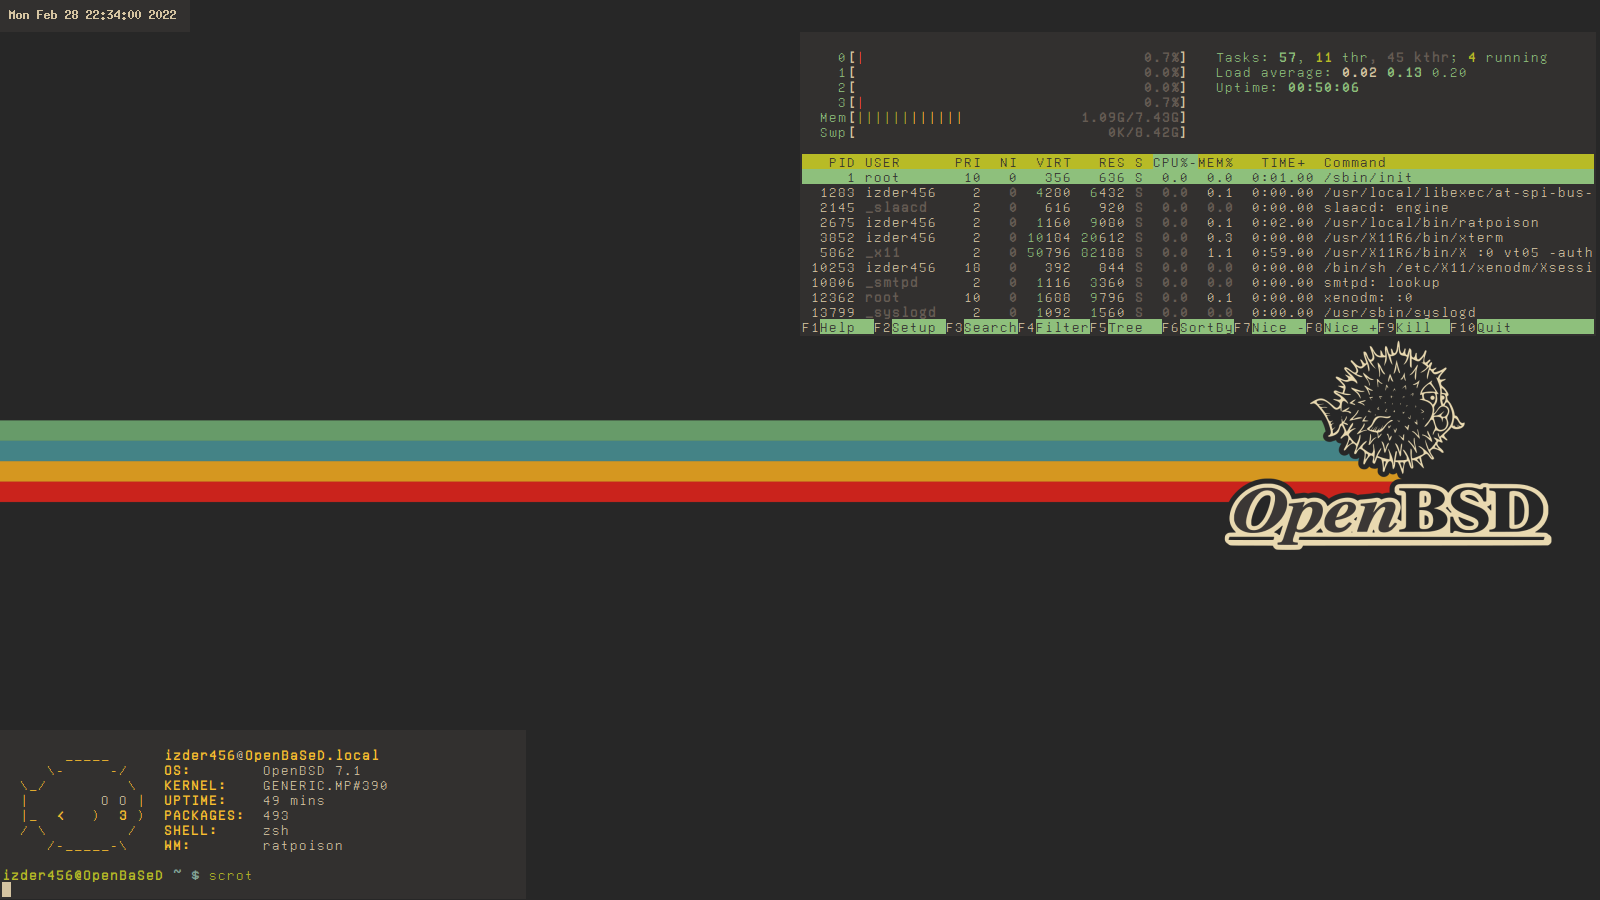
\includegraphics[width=0.8\textwidth]{imagens/desktop.png}
    \caption{Captura de tela do \href{https://www.reddit.com/r/unixporn/comments/t3zgiu/ratpoison_lightweight_openbsdcurrent_gruvbox/}{\textit{/u/
Izder456} na \textit{/r/unixporn}}}
\end{figure}

É importante que tenha prazer na leitura de manuais, já que para alcançar algo semelhante a imagem acima, será preciso conhecimento de ferramentas de monitoramento de rede, tela, energia, E/S etc. Além disto, pode ser necessária a compilação de diversos programas não inclusos nos repositórios do OpenBSD. Outra alternativa, seria utilizar o Xfce, que é mais simples de obter neste sistema operacional, para tal, basta os seguintes pacotes: \verb|xfce| e \verb|xfce-extras| e algumas configurações na inicialização do sistema.

\begin{figure}[!ht]
    \centering
    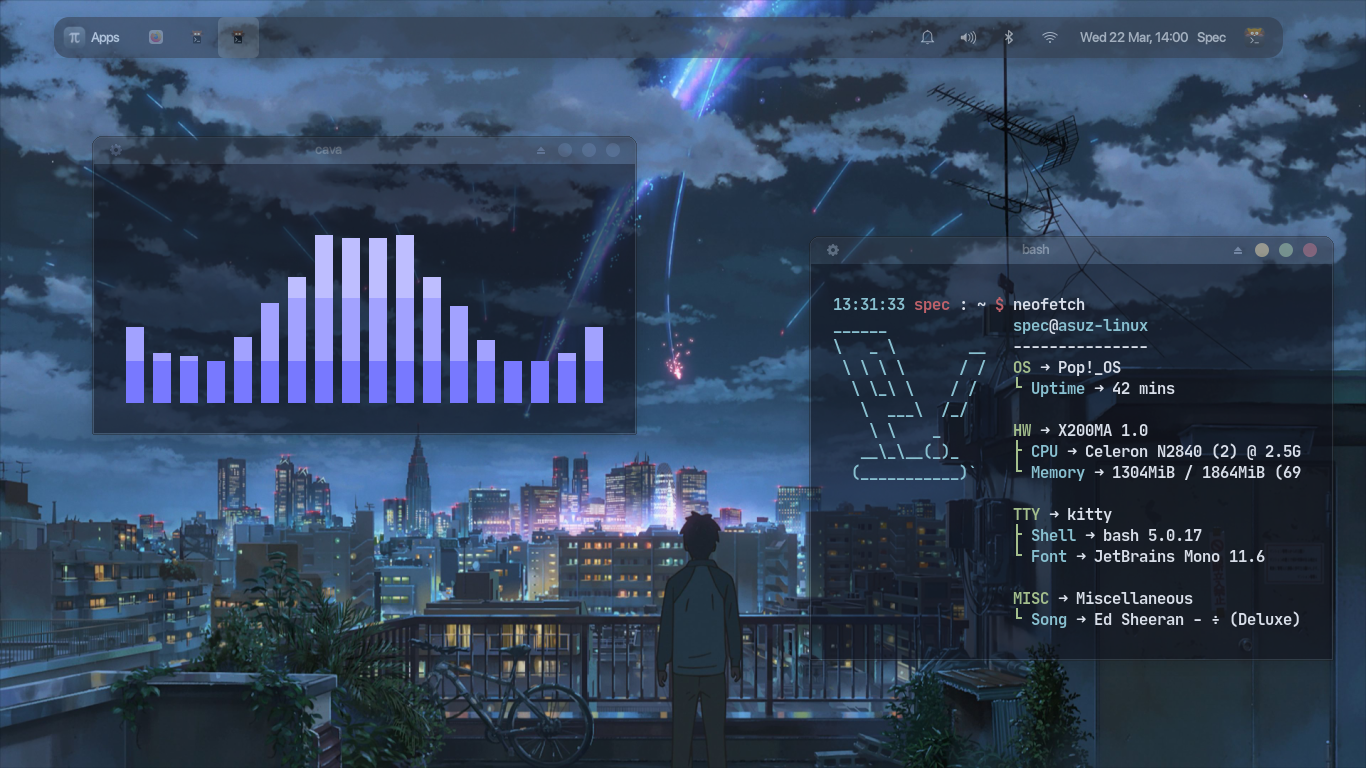
\includegraphics[width=0.8\textwidth]{imagens/xfce.png}
    \caption{Xcfe altamente configurado de \href{https://www.reddit.com/r/unixporn/comments/11yc4d2/xfce_first_xfce_rice/}{\textit{/u/Smart\_Main6779} na \textit{/r/unixporn}}}
\end{figure}

Há outros ambientes gráficos completos, como GNOME e KDE Plasma, mas não são completamente compatíveis com o OpenBSD, ao menos com suas últimas novidades como o uso do \textit{Wayland}. Além do mais, possuem maior integração com sistemas GNU/Linux devido suas tecnologias e maior apoio comunitário e corporativo.

\section{Conclusão}

Além disso, o OpenBSD não se contenta apenas em proteger os usuários dentro de seu próprio ecossistema. Com o desenvolvimento de ferramentas como OpenSSH e PF, o OpenBSD estendeu sua influência muito além de suas próprias fronteiras, contribuindo para um ambiente de tecnologia mais seguro como um todo.

Ainda assim, o OpenBSD não é apenas um sistema operacional seguro, é também um sistema operacional inovador. As suas práticas de desenvolvimento e as soluções que cria não só protegem os usuários, mas também estimulam a indústria a seguir seu exemplo, elevando o padrão de segurança em todo o setor de tecnologia.

O mundo tecnológico é complexo e cheio de desafios. No entanto, sistemas operacionais como o OpenBSD ilustram que com um compromisso inabalável com a segurança, a inovação e a qualidade do código, é possível criar um ambiente digital mais seguro. Ao fazer isso, o OpenBSD não apenas protege seus próprios usuários, mas contribui para a melhoria da saúde digital global, tornando a nossa vida conectada um pouco mais segura.

O OpenBSD é mais do que um sistema operacional: é um farol de segurança, qualidade e inovação, iluminando o caminho para um futuro digital mais seguro. Concluímos assim nossa jornada, com a esperança de que essa exploração tenha proporcionado uma apreciação mais profunda do OpenBSD e da importância crucial de sua missão na era digital.

\begin{figure}[!ht]
    \centering
    
\includegraphics[width=0.6\textwidth]{imagens/openbsd-logo.png}
\end{figure}

\printbibliography
\end{document}
